\chapter{CEM Source Language}

For a better grasp on what the cem native code compiler can do, I share a
number of example programs and libraries. I highlight the fact that the compiler
can handle machine literals and primitive operations, including system calls and
a basic system for monadic side effects.  There are a number of non-standard
design decisions worth mentioning. The first, and most significant one, is a
non-standard use of parentheses. Instead of implicit applications, we use
\texttt{()} parentheses to explicitly denote left-associative applications, and
\texttt{\[\]} brackets to denote explicit right-associative applications. We use
either the unicode $\lambda$ character or the forward slash \texttt{\\x.b} to
denote lamdas, where \texttt{x} is a variable and \texttt{b} is the body of the
lambda. This choice of explicit applications simplifies the syntax in a way that
prevents ambiguity and simplifies parsing. 

\section{Prelude}
An extremely useful tool for any language is a base set of functionality
available in global namespace. I follow Haskell terminology and refer to this
set of bound variables as a Prelude. 

\subsection{Pure Prelude}
I start with a pure fragment of the prelude: there are no partial functions
modulo termination and type-safety. Note we have wrapper functions for our
machine primitive operations that force evaluation of arguments. We also make
heavy use of right-associative applications, wrapped with square brackets
\texttt{[]}. This is in contrast to using an infix operator, e.g. the $\$$
operator in Haskell.

Also note that we define the y-combinator at the start of the prelude; this is
the source of all recursion. Whether or not this is sufficient for all
call-by-need recursion seems to be a topic for disagreement \cite{ariola}, but
we have found it to be quite useful in     

\begin{verbatim}
# Recursion!
Y = \g.(\x.[g x x] \x.[g x x])

# Boolean integer comparisons
= = \n.\m.\t.\f.[m n \n.\m._=]
!= = \n.\m.\t.\f.[m n \n.\m._\=]
>= = \n.\m.\t.\f.[m n \n.\m._>=]
<= = \n.\m.\t.\f.[m n \n.\m._<=]
< = \n.\m.\t.\f.[m n \n.\m._<]
> = \n.\m.\t.\f.[m n \n.\m._>]

# Arithmetic
+ = \n.\m.[m n \n.\m._+]
- = \n.\m.[m n \n.\m._-]
-' = (0 -)
* = \n.\m.[m n \n.\m._*]
/ = \n.\m.[m n \n.\m._/]
% = \n.\m.[m n \n.\m._%]
^ = \n.(Y \^.\l.\n*.\m.(m = 0 n* (^ (n * n*) (m - 1))) n 1)

# Booleans
false = \t.\f.f
true = \t.\f.t
and = \a.\b.(a b false)
or = \a.\b.(a true b)
not = \a.(a false true)

# Maybe
Nothing = \n.\j.n
Just = \a.\n.\j.(j a)

# Either 
Left = \v.\l.\r.(l v)
Right = \v.\l.\r.(r v)

# Lists
cons = \h.\t.\n.\c.(c h t)
: = cons
nil = true
; = nil
null = \l.(l true \h.\t.false)

# Tuple
pair = \f.\s.\p.(p f s)
fst = \p.(p \x.\y.x)
snd = \p.(p \x.\y.y)
uncurry = \f.\p.(p f)

# Monad
>>= = \c.\f.\w.(c w f)
>> = \c.\f.\w.(c w \v.f)
return = pair
when = \b.\a.(b a (return 0))

# Misc
gcd = (Y \gcd.\a.\b.([b 0 =] a (gcd b [a b %])))
lcm = \a.\b.(a * b / (gcd a b))
even = \n.(n % 2 = 0)
odd = \n.(n % 2 = 1)
id = \x.x
const = true
compose = \f.\g.\x.[f g x]
flip = \f.\b.\a.(f a b)
until = (Y \until.\p.\f.\x.(p x x (until p f (f x)))) 
map = (Y \map.\f.\xs.(xs nil \h.\t.(cons (f h) (map f t))))
length = \xs.(Y \length.\xs.\acc.(xs acc \h.\t.(length t (acc + 1))) xs 0)
foldl = (Y \foldl.\f.\a.\bs.(bs a \b.\bs.(foldl f (f a b) bs)))
foldr = (Y \foldr.\f.\a.\bs.(bs a \b.\bs.(f b (foldr f a bs))))
append = \as.\bs.(foldr cons bs as)
++ = append
reverse = (foldl (flip cons) nil) 
any = \p.\xs.(foldr or false (map p xs))
all = \p.\xs.(foldr and true (map p xs))
concat = (foldr append nil)
concatMap = \f.(foldr (compose append f) nil)
filter = \c.(Y \filter.\ls.(ls nil \h.\t.(c h (cons h) id (filter t))))
scanl = (Y \scanl.\f.\q.\ls.(cons q (ls nil \x.\xs.(scanl f (f q x) xs))))
scanr = (Y \scanr.\f.\q.\ls.(ls (cons q nil) \x.\xs.(scanr f x q nil \q.\qs.(cons (f x q)))))
iterate = (Y \iterate.\f.\x.(cons x (iterate f (f x))))
repeat = (iterate id)
take = (Y \take.\n.\xs.(xs ; \x.\xs.(n <= 0 ; (: x (take (n - 1) xs)))))
replicate = \n.\x.(take n (repeat x))
cycle = \xs.[concat repeat xs]
drop = (Y \drop.\n.\xs.(xs ; \x.\xs.(n = 1 xs (drop (n - 1) xs))))
tail = (drop 1)
splitAt = \n.\xs.(pair (take n xs) (drop n xs))
takeWhile = (Y \takeWhile.\f.\xs.(xs nil \x.\xs.(f x (cons x (takeWhile f xs)) nil)))
dropWhile = (Y \dropWhile.\f.\xs.(xs nil \x.\xs.(f x (dropWhile f xs) (cons x xs))))
splitHalf = (Y \sh.\xs.(xs (pair ; ;) \h1.\t1.(t1 (pair (: h1 ;) ;) \h2.\t2.
  {tails = (sh t2)} (tails \f.\s.(
  (pair (: h1 f) (: h2 s)))))))
sort = \f.{merge = (Y \merge.\xs.\ys.(xs ys \x.\xts.(ys xs \y.\yts.(f x y 
             (: x (merge xts ys)) (: y (merge xs yts))))))}
  (Y \ms.\l.(length l < 2 l (splitHalf l \f.\s.(merge (ms f) (ms s)))))
split = \f.(Y \split.\xs.(xs (pair nil nil) \h.\t.(f h 
  (pair nil t)
  (split t \acc.\rem.(pair (cons h acc) rem)))))
showInt = \i.{showPosInt = (compose reverse (Y \showPosInt.\i.(i = 0
    nil 
    (cons (i % 10 + 48) (showPosInt (i / 10))))))} [
  (i = 0 "0") 
  (i < 0 (cons '-' (showPosInt (0 - i))))
  (showPosInt i)
]
readInt = (compose (Y \readInt.\n.(n 0 \h.\t.(h - 48 + (readInt t * 10))))
  (compose reverse (takeWhile \h.(and (h >= 48) (h < 58)))))
showBool = \b.(b "true" "false")
forever = \c.(Y \forever.(>> c forever))
isSpace = \c.(any (= c) " \n\t\r")
partition = \f.(Y \partition.\s.\acc.(s (pair acc nil) \h.\t.(f h (pair acc s)
    (partition t (append acc))))) 
splitWhen = \f.(Y \splitWhen.\xs.(split f xs \l.\r.(r 
  (l ; \h.\t.(: l ;))
  \h.\t.{cont = (splitWhen r)}(l cont \h.\t.(: l cont)))))
words = (splitWhen isSpace)
lines = (splitWhen (= '\n'))
splitArgs = (map (map fst) (splitWhen \p.(p \e.\c.(and (not e) (c = ' '))) 
  (drop 1 (scanl \q.\x.(q \p.\c.(c = '\\' (pair true x) (pair false x))) (pair false ' ')))))
intersperse = \v.(Y \intersperse.\l.(l l \h.\t.(t l 
  \h'.\t'.[(: h) (: v) intersperse t])))
unwords = (compose concat (intersperse " "))
if = id
from = (iterate (+ 1))
range = \s.\e.(take (e - s + 1) (from s))
then = \cont.\result.cont
sum = (foldr + 0)
max = \x.\y.(x > y x y)
min = \x.\y.(x < y x y)
unlines = (concatMap (flip append "\n"))
apply = (Y \al.\f.\l.(l f \h.\t.(al (f h) t))) 
signum = \n.(n = 0 0 (n > 0 1 (-' 1)))
abs = \n.(n < 0 (0 - n) n)
zipWith = \f.(Y \zipWith.\as.\bs.(as nil \a.\at.(bs nil \b.\bt.
  (: (f a b) (zipWith at bt)))))
zip = (zipWith pair)
for = \as.\f.(Y \for.\as.(as (return id) \a.\as.(>> (f a) (for as))) as)
mapm_ = (flip for)
mapm = \f.\as.(Y \mapm.\as.\acc.(as (return acc) \a.\as.(>>= (f a) \c.(mapm as (cons c acc)))) as nil)
replace = \l.\v.(map (const v) l)
zip-with-default = \f.\d.(Y \zwd.\as.\bs.(as 
  (replace bs d)
  \a.\at.(bs 
    (replace as d)
    \b.\bt.(: (f a b) (zwd at bt)))))
strcmp = \s1.\s2.(all id (zip-with-default = false s1 s2))
lookup = \elem.\eqfun.(Y \lookup.\l.(l 
  Nothing 
  \h.\t.(h \key.\value.(eqfun elem key
    (Just value)
    (lookup t)))))
elem = \val.\func.\list.(lookup val func list false true)
\end{verbatim}

\subsection{Side Effects and Partial Functions}
A necessary feature of a real world programming language is the ability to have
side effects. Here we define a small set of basic tools for implementing basic
side effects, including memory reads and writes, and system calls. Note we take
an approach that avoids depending on \texttt{libc}, implementing analogous
functionality directly in lambda calculus with access to system calls. 

For modeling side effects in lambda calculus, we take an approach inspired by
the IO monad in Haskell. We extend our language with an object of type real
world, and have our side-effectful functions consume and generate a new
real-world value. This allows us to implement and use the monad bind and return
functions directly. While we don't have infix operators or Haskell's
do-notation, writing imperative programs is still entirely possible, though
certainly more clunky. 

\begin{verbatim}
## Memory read and write wrappers ##
mvq = \val.\addr.\w.[w addr val \a.\b.\w._@q]
rdq = \addr.\w.[w addr \a.\w._$q]
mvl = \val.\addr.\w.[w addr val \a.\b.\w._@l]
rdl = \addr.\w.[w addr \a.\w._$l]
mvs = \val.\addr.\w.[w addr val \a.\b.\w._@s]
rds = \addr.\w.[w addr \a.\w._$s]
mvb = \val.\addr.\w.[w addr val \a.\b.\w._@b]
rdb = \addr.\w.[w addr \a.\w._$b]
mv = mvq
rd = rdq

## System calls ##
sys_mmap = \addr.\len.\prot.\flags.\fd.\offset.\w.[w 9 offset fd flags prot len addr \a.\b.\c.\d.\e.\f.\t.\w._!6]
sys_write = \fd.\buf.\count.\w.[w 1 count buf fd \a.\b.\c.\t.\w._!3]
sys_read = \fd.\buf.\count.\w.[w 0 count buf fd \a.\b.\c.\t.\w._!3]
sys_open = \fname.\flags.\mode.\w.[w 2 mode flags fname \a.\b.\c.\t.\w._!3]
sys_close = \fd.\w.[w 3 fd \a.\t.\w._!1]
sys_exit = \code.\w.[w 60 code\a.\t.\w._!1]
sys_socket = \dom.\type.\prot.\w.[w 41 prot type dom \a.\b.\c.\t.\w._!3]
sys_getpid = \w.[w 39 \t.\w._!0]
sys_fork = \world.[world 57 \t.\w._!0]
sys_nanosleep = \rqtp.\rmtp.\w.[w 35 rmtp rqtp \a.\b.\t.\w._!2]
sys_munmap = \addr.\len.\w.[w 11 len addr \a.\b.\t.\w._!2]
sys_wait = \pid.\w.[w 61 0 0 pid \pid.\a.\b.\t.\w._!3]
sys_execve = \fname.\argv.\envp.\w.[w 59 envp argv fname \a.\b.\c.\t.\w._!3]
sys_getdents = \fd.\dirent*.\count.\w.[w 78 count dirent* fd \a.\b.\c.\t.\w._!3]

## Basic IO ##
pageSize = 4096
malloc = \len.(sys_mmap 0 len 255 34 (-' 1) 0)
free = \ptr.(sys_munmap ptr 1)
sleep = \sec.\nsec.(>>= (malloc 2) \p.
  (>> (mvq sec p) 
  (>> (mvq nsec (p + 8)) 
  (>>= (sys_nanosleep p p) \r.
  (free p)))))
newPage = (malloc pageSize)
read-utf8-char-from-buf = \p.(>>= (rdb p) \c1.
  (c1 / 128 = 0 (return (pair c1  1)) (>>= (rdb (p + 1)) \c2.{c2' = (2 ^ 8 * c2 + c1)}
  (c2 / 128 = 0 (return (pair c2' 2)) (>>= (rdb (p + 2)) \c3.{c3' = (2 ^ 16 * c3 + c2')}  
  (c3 / 128 = 0 (return (pair c3' 3)) (>>= (rdb (p + 3)) \c4.
  (return (pair (2 ^ 24 * c4 + c3') 4)))))))))
write-utf8-char-to-buf = \c.\p.[
  (c <= 0x7f (>> (mvb c p) (return 1)))
  (c <= 0x7ff (>> (mvb (c / 0x40 + 0xc0) p) 
              (>> (mvb (c % 0x40 + 0x80) (p + 1)) (return 2))))
  (c <= 0xffff (>> (mvb (c / 0x1000 + 0xe0) p)
               (>> (mvb (c % 0x1000 / 0x40 + 0x80) (p + 1))
               (>> (mvb (c % 0x40 + 0x80) (p + 2))
               (return 3)))))
  (>> (mvb '?' p) (return 1))]
readStrBuf = (Y \rstr.\loc.\n.(n = 0
  (return nil)
  (>>= (read-utf8-char-from-buf loc) \p.(p \c.\n'.
  (>>= (rstr (loc + n') (n - n')) \s.(return (: c s)))))))
readStrBuf' = (Y \rstr.\loc.
  (>>= (read-utf8-char-from-buf loc) \p.(p \c.\n'.
  (c = 0
  (return nil)
  (>>= (rstr (loc + n')) \s.(return (: c s)))))))
putStrBuf = \size.\buf.{
  putStrBuf = (Y \putStrBuf.\loc.\s.
  {finished = (return (pair loc s))}
  (s 
    finished 
    \h.\t.(loc - buf >= (size - 4) # This is to ensure the 4 byte unicode char can't be written
      finished 
      (>>= (write-utf8-char-to-buf h loc) \n.(putStrBuf (loc + n) t)))))
  }
  (putStrBuf buf)
open = \fname.(>>= newPage \nameBuf.(
  >> (putStrBuf pageSize nameBuf fname)
  (sys_open nameBuf 66 0)))
openrd = \fname.(>>= newPage \nameBuf.(
  >> (putStrBuf pageSize nameBuf fname)
  (sys_open nameBuf 0 0)))
putPtrBuf = (Y \putPtrBuf.\loc.\s.(s 
  (>> (mv 0 loc) (return (loc + 8)))
  \h.\t.(>> (mv h loc) (putPtrBuf (loc + 8) t))))
readPtrBuf = (Y \rstr.\loc.\n.(n <= 0
  (return nil)
  (>>= (rd loc) \p.(p = 0
    (return nil)
    (>>= (rstr (loc + 8) (n - 1)) \s.(return (: p s)))))))
writeFd = \fd.\str.(>>= newPage \iobuf.(>> (Y \writeFd.\str.
  (>>= (putStrBuf pageSize iobuf str) \p.(p \p.\s.
  (>>= (sys_write fd iobuf (p - iobuf)) \n.
  (nil? s (return n) (writeFd s))))
) str) (free iobuf)))
writeFile = \fname.\str.(newPage >>= \iobuf.(
  >>= (open fname) \fd.(
  >> (fd > 1024 (sys_exit 2) (writeFd fd str))
  (free iobuf))))
readFd = \fd.(>>= newPage \iobuf.(Y \readFd.
  (>>= (sys_read fd iobuf pageSize) \n.
  (>>= (readStrBuf iobuf n) \s.
  (n < pageSize
    (return s)
    (nil? s
      (return nil)
      (>>= readFd (compose return (append s)))))))))
readFile = \fname.(>>= (openrd fname) \fd.
  (or (fd > 1024) (fd < 0)
    (sys_exit (-' 1))
    (readFd fd)))
putStr = (writeFd 1)
putStrLn = \s.(writeFd 1 (append s "\n"))
print = putStrLn
getContents = (readFd 0)
getLine = (>>= getContents \s.(return (takeWhile (!= '\n') s)))
interact = \f.(>>= getContents (compose putStr f))

# Prelude-like utilities that require IO, e.g. partial functions
fork = \c.(>>= sys_fork \n.(n = 0 (>> c (sys_exit 0)) (sys_wait n)))
error = \s.(>> (putStrLn s) (sys_exit 1) 0)
undefined = (error "undefined")
PME = (error "Pattern match error")
head = \l.(l (error "head of empty list") \h.\t.h)
index = \n.\k.(Y \index.\n.\k.\cont.(n = 0
  cont
  \x.(index (n - 1) k (k = n x cont))) n (n - k + 1) (error "index failed"))
listIndex = (Y \listIndex.\n.\l.(l (error "listIndex failed") \h.\t.(n = 0 h (listIndex (n - 1) t))))
!! = listIndex
fst = (index 2 1)
snd = (index 2 2)
sprintf_ = \k.(Y \printf.\acc.\l.(l (k acc) \h.\t.(h = '%'
  (t (append acc "%") \h.\t'.[
    (h = 'd' \i.(printf (append acc (showInt i)) t'))
    (h = 'c' \c.(printf (append acc (cons c nil)) t'))
    (h = 's' \s.(printf (append acc s) t'))
    (h = 'b' \b.(printf (append acc (showBool b)) t'))
    (printf (append acc "%") t)])
  (printf (append acc (cons h nil)) t))) nil)
sprintf = (sprintf_ id)
printf = (sprintf_ print)
trace = \x.(sprintf_ print 0 \w.\s.x)
putWords = (Y \putWords.\ws.\startloc.(ws
  (return (pair startloc nil))
  \w.\ws.
    (>>= (putStrBuf pageSize startloc (++ w (: 0 ;))) \p.(p \endloc.\str.
    (>>= (putWords ws endloc) \p.(p \ptrloc.\ws.
    (return (pair ptrloc (cons startloc ws)))))))))
getArgs = (>>= sys_getpid \i.{fname = (sprintf "/proc/%d/cmdline" i)}
  (>>= (readFile fname) \s.[return tail [splitWhen = 0] s]))
getEnv = (>>= sys_getpid \i.{fname = (sprintf "/proc/%d/environ" i)}
  (>>= (readFile fname) \s.{bindings = (splitWhen (= 0) s)}
  (return (map (split (= '=')) bindings))))
getRawEnv = (>>= sys_getpid \i.{fname = (sprintf "/proc/%d/environ" i)}
  (>>= (readFile fname) \s.{bindings = (splitWhen (= 0) s)}
  (return bindings)))
# LS 
d_ino = \ld.(rdl ld)
d_off = \ld.(rdl (ld + 8))
d_reclen = \ld.(rds (ld + 16))
d_name = \ld.(ld + 18)

# String -> IO [String]
ls = \path.(>>= newPage \buf.
  (>> (putStrBuf pageSize buf path) 
  (>>= (sys_open buf 0x10000 0) \fd.
  (fd < 0 
    (>> (printf "%s is not a directory" path)
    (return nil))
  (>>= (sys_getdents fd buf pageSize) \n.
  (n < 0 
    (>> (printf "getdents on directory \"%s\" failed with errno %d" path n)
    (return nil))
  {read-dent = (Y \rdd.\ld.(ld - n >= buf
      (return nil)
    (>>= (d_ino ld) \ino.
    (>>= (d_off ld) \off.
    (>>= (d_reclen ld) \reclen.
    (>>= (readStrBuf' (d_name ld)) \name.
    (>>= (rdd (ld + reclen)) \names.
    (return (cons name names)))))))))
  }
  (>>= (read-dent buf) \files.
  (>> (free buf)
  (return files)))))))))
pwd = (>>= getEnv \env.(lookup "PWD" strcmp env (return "/") return))
findPath = \name.(>>= getEnv \env.
  {paths = (lookup "PATH" strcmp env (cons "/usr/bin" nil) (splitWhen (= ':')))}
  {find-file = (Y \ff.\paths.(paths (>> (printf "couldn\'t find %s" name) (return name)) \p.\ps.(>> (printf "checking %s")
    (>>= (ls p) \fs.(elem name strcmp fs (>> (printf "found %s in %s" name p) (return (append p (cons '/' name)))) (>> (printf "couldn\'t find %s in %s" name p) (ff ps)))))))}
  (find-file paths))
exec = \str.(splitArgs str (return 0) \fname.\argv.
  (>>= getEnv \env.
  (>> (printf "running %s with args: " fname)
  (>> (mapm_ putStr argv) (>> (print ".")
  (>>= (elem '/' = fname (return fname) (findPath fname)) \fullname.
  (>>= newPage \buf.
  (>>= (putStrBuf pageSize buf (++ fullname (: 0 ;))) \p.(p \l.\str.
  (>>= (putWords argv l) \p.(p \al.\alocs.
  (>>= (putPtrBuf al (cons buf alocs)) \l.
  (>>= getRawEnv \env.
  (>>= (putWords env l) \p.(p \el.\elocs.
  (>>= (putPtrBuf el elocs) \l.
  (>>= (sys_execve buf al el) \retval.
  (>> (free buf)
  (return retval)))))))))))))))))))
system = (compose fork exec)
\end{verbatim}

Note the use of parentheses gets pretty hairy. Despite our right associative
applications, the lack of infix operators and do-notation hurts the readiability
of long imperative programs significantly. Still, it is certainly
\emph{possible} to write programs in this style. Note also that our heavy use of
newPage shows that our lack of stack allocated memory is a pain. Due to our use
of the system stack for our argument closures and update markers, incorporating
alloca-style stack allocations would be a significant challenge, though it
should be possible. 

\section{Example Programs}

In addition to re-writing the no-fib benchmark suite, we started writing example
programs in this source language to gauge the difficulty. These programs use the
prelude described above to implement basic programs. 

We start with a canonical example of using call-by-need to implement a
dynamic programming linear time fibonacci. 

\begin{verbatim}
fibs = (Y \fibs.[(1 :) (1 :) (zipWith + fibs (tail fibs))])
\end{verbatim}

This is an interesting example, because unlike the similar Haskell
implementation, this implementation is \emph{guaranteed} to run in linear time.
Because Haskell is a \emph{non-strict} language, we rely on its use of
call-by-need as an optimization technique, not a guaranteed property of the
language. Note also the the infix use of \texttt{:}. This is possible due to the
implementation of machine integers. Recall that we don't have algebraic data
types, so the technique used by Haskell of wrapping machine literals in a
\texttt{newtype} is not an option. Instead, we use evaluation to force the
value. In place of an environment pointer, we place the machine literal, and use
the code pointer to take the continuation and apply itself to it. In this case,
that results in the cons constructor applying itself to the value 1. Note that
this is the approach used in all the machine primitive operations in the prelude
listed above as well. While this is operationally equivalent the Haskell
approach, it does raise questions about referential transparancy.    

Another simple example shows how we can use the fork system call to implement
parallel programs. This shows how easy it is to use the IO monad without the use
of type classes. 

\begin{verbatim}
main = (>>= sys_fork \r.(r = 0
  (print "Child says hi")
  (print "Parent says hi")))
\end{verbatim}

Note again we use the fact that forcing \texttt{r} before checking equality is a
perfectly valid thing to do, though not necessary in this case as the equality
check \texttt{=} will force it as well. 

\section{Visualization}

In addition to the native code compiler, I have implemented a graphviz-based
visualization tool that helps visualize how the heap changes over time. It uses
variable names in the heap instead of deBruijn indices to increase readability.
It also shows the stack and current closure through steps of the small step \ce
semantics. The primary use is just to see how the cactus structure evolves
through evaluation, and how it ensures sharing. 

For example, consider evaluation of the expression

\begin{verbatim}
(\a.(\b.(b a) \c.(c a)) (\i.i \j.j))
\end{verbatim}

By running the \texttt{cem} executable with the flags \texttt{-pg}, we get the
following output: 

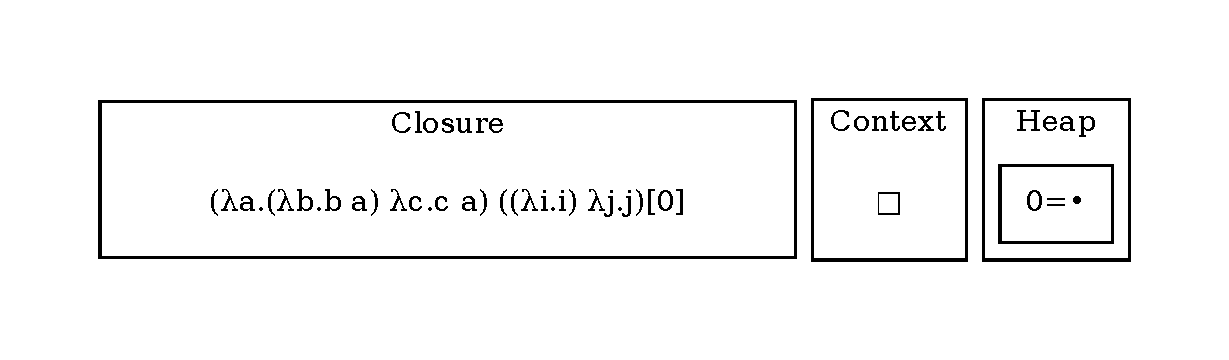
\includegraphics[width=\linewidth/2]{figures/1.pdf}
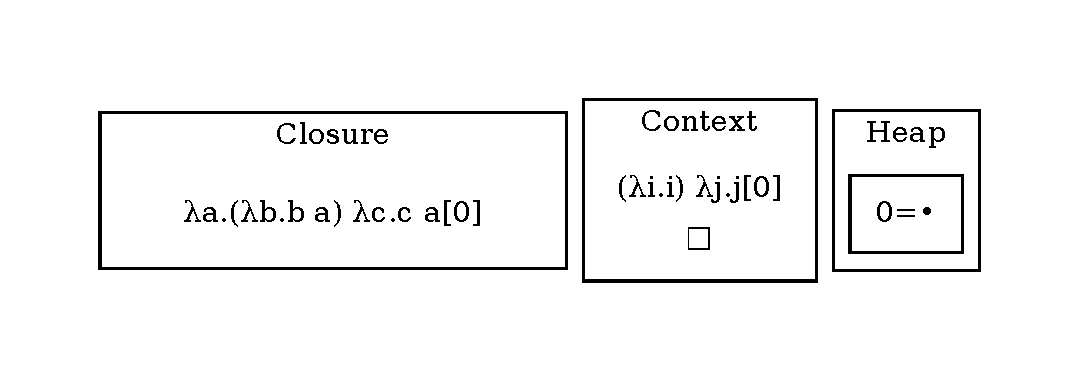
\includegraphics[width=\linewidth/2]{figures/2.pdf}
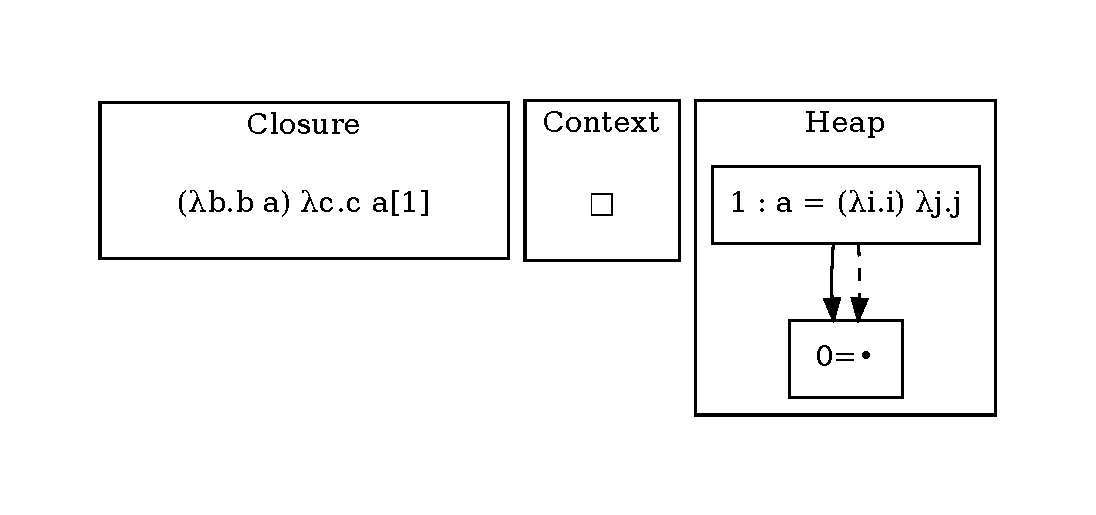
\includegraphics[width=\linewidth/2]{figures/3.pdf}
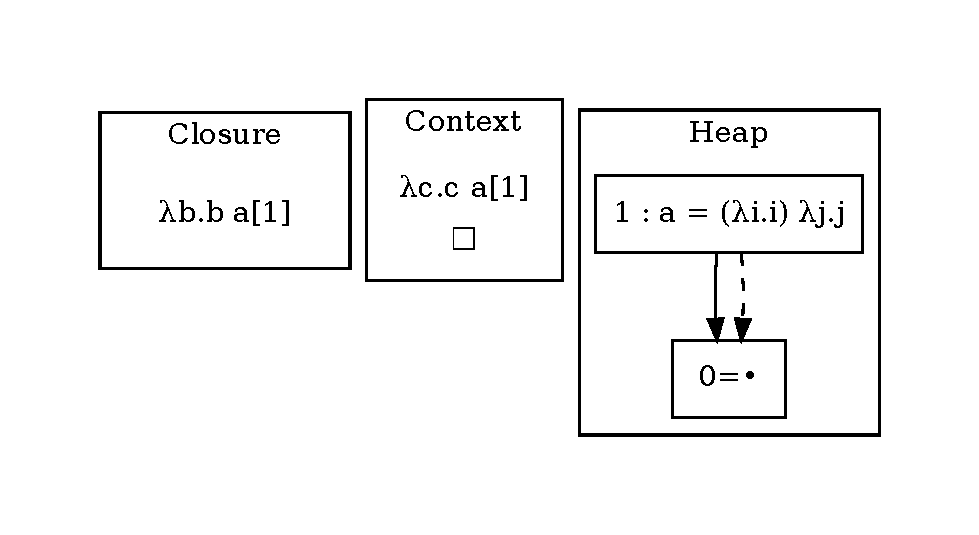
\includegraphics[width=\linewidth/2]{figures/4.pdf}
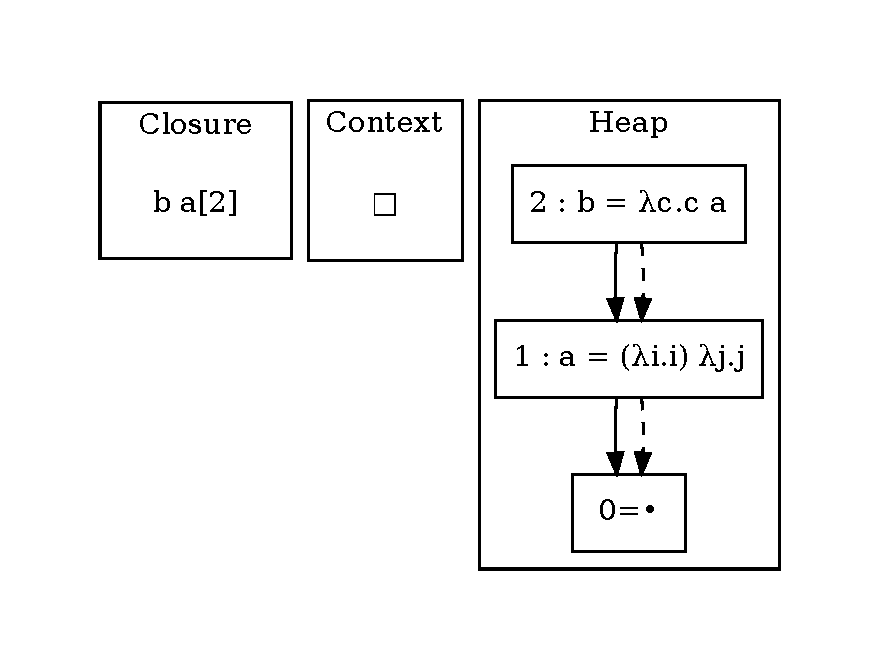
\includegraphics[width=\linewidth/2]{figures/5.pdf}
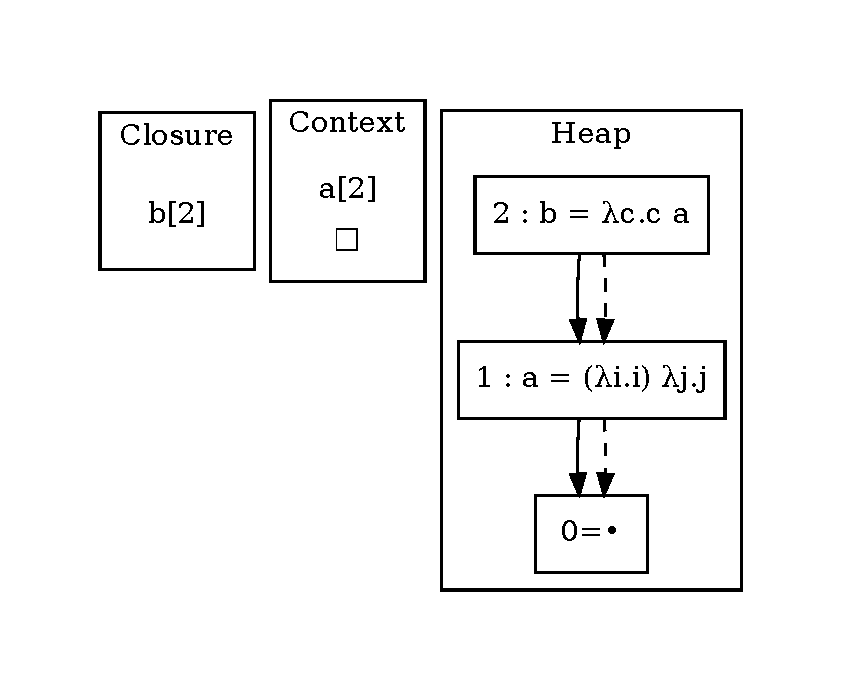
\includegraphics[width=\linewidth/2]{figures/6.pdf}
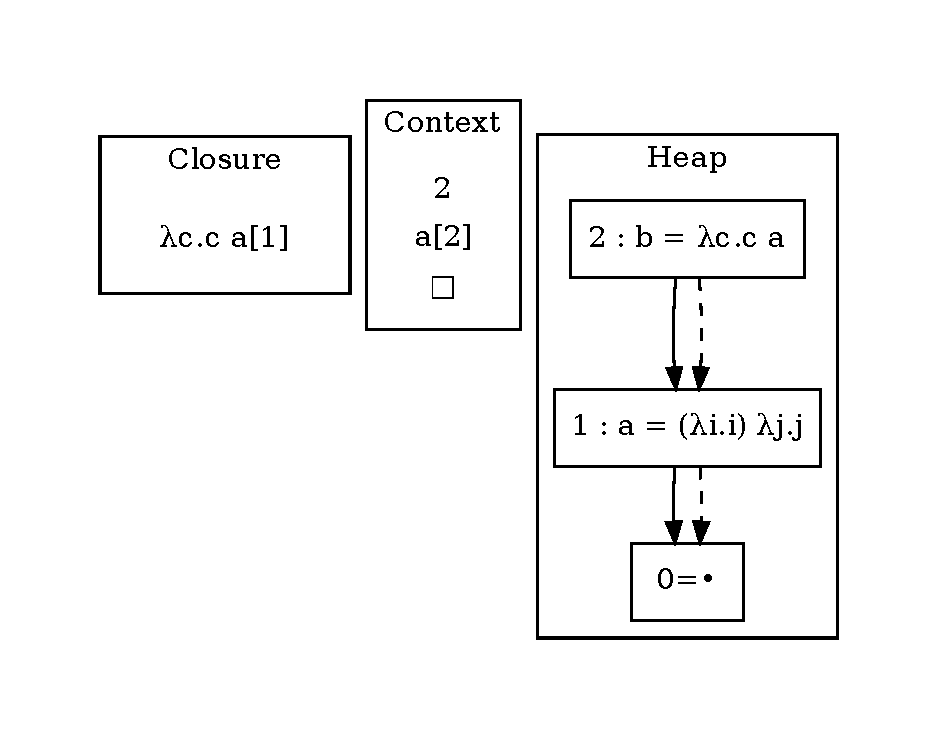
\includegraphics[width=\linewidth/2]{figures/7.pdf}
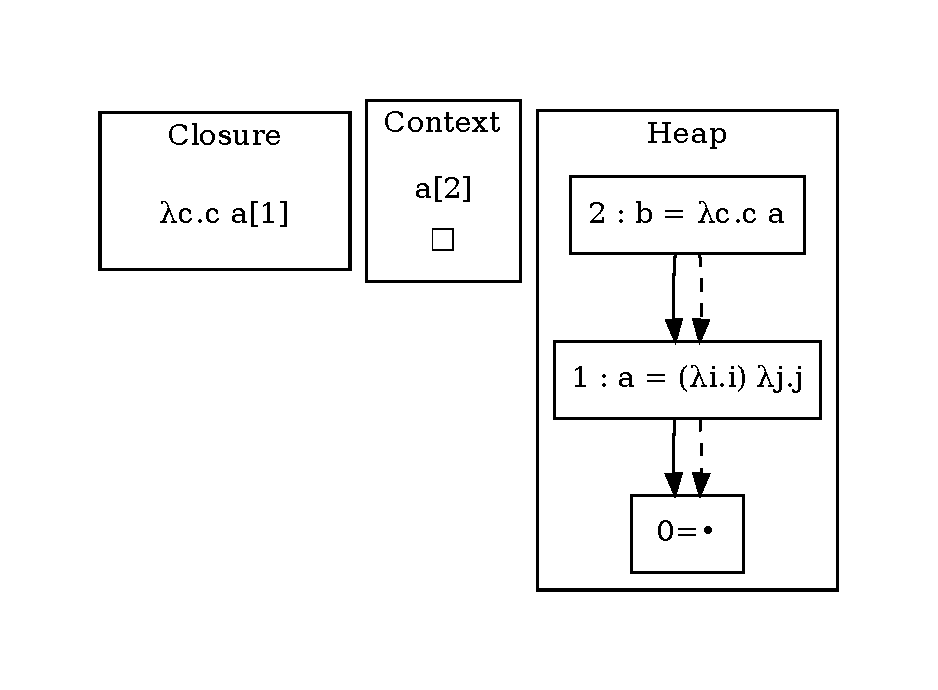
\includegraphics[width=\linewidth/2]{figures/8.pdf}
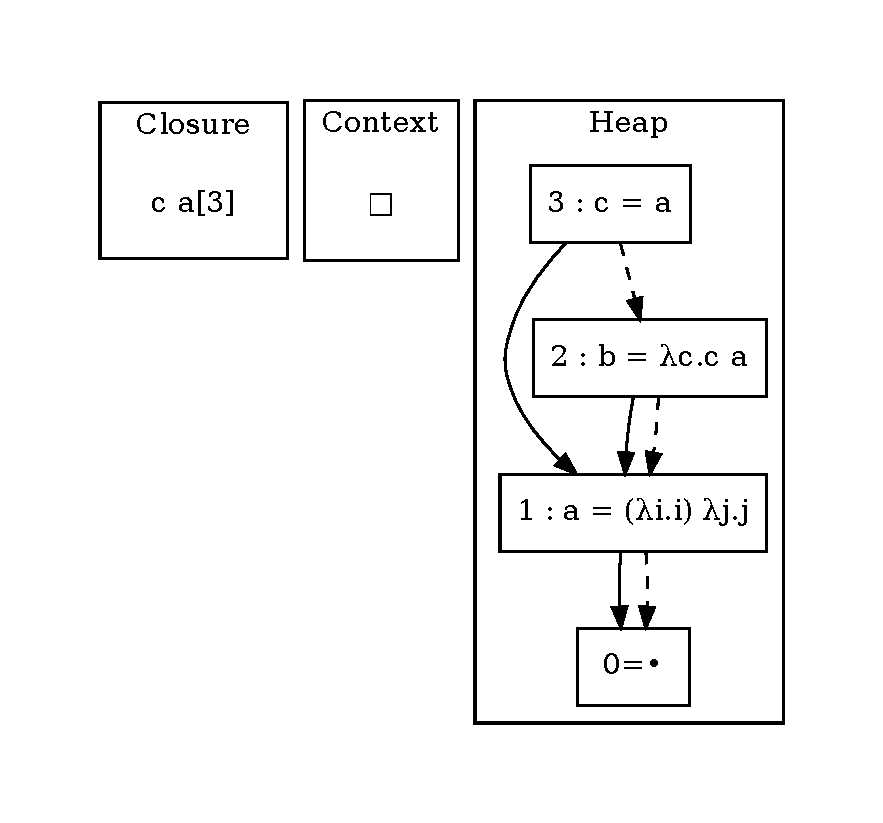
\includegraphics[width=\linewidth/2]{figures/9.pdf}
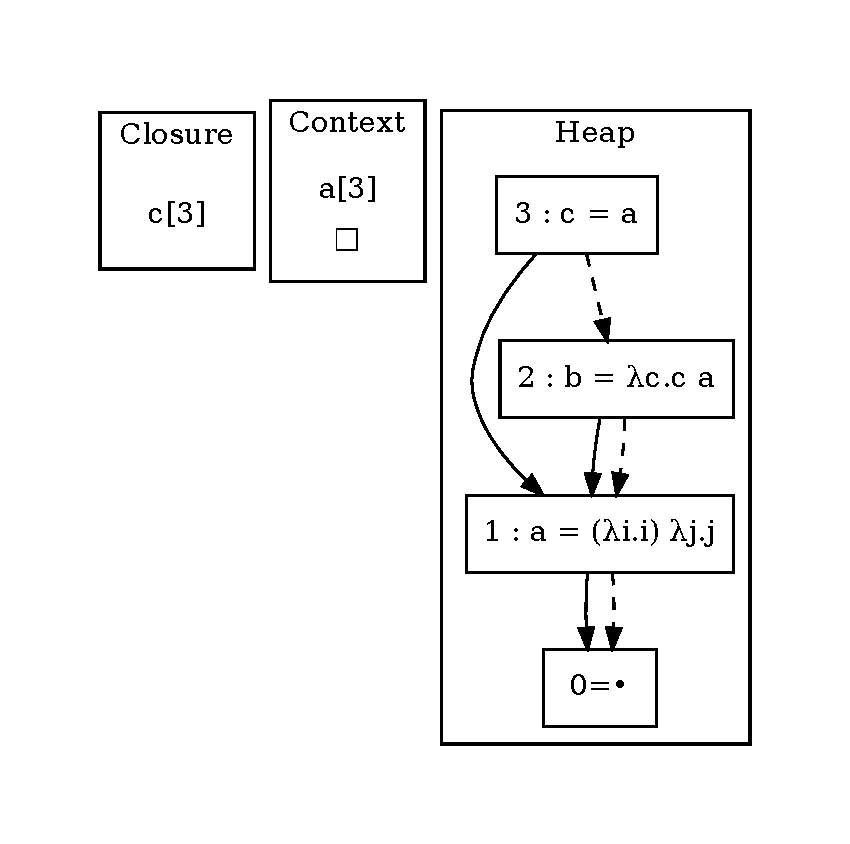
\includegraphics[width=\linewidth/2]{figures/10.pdf}
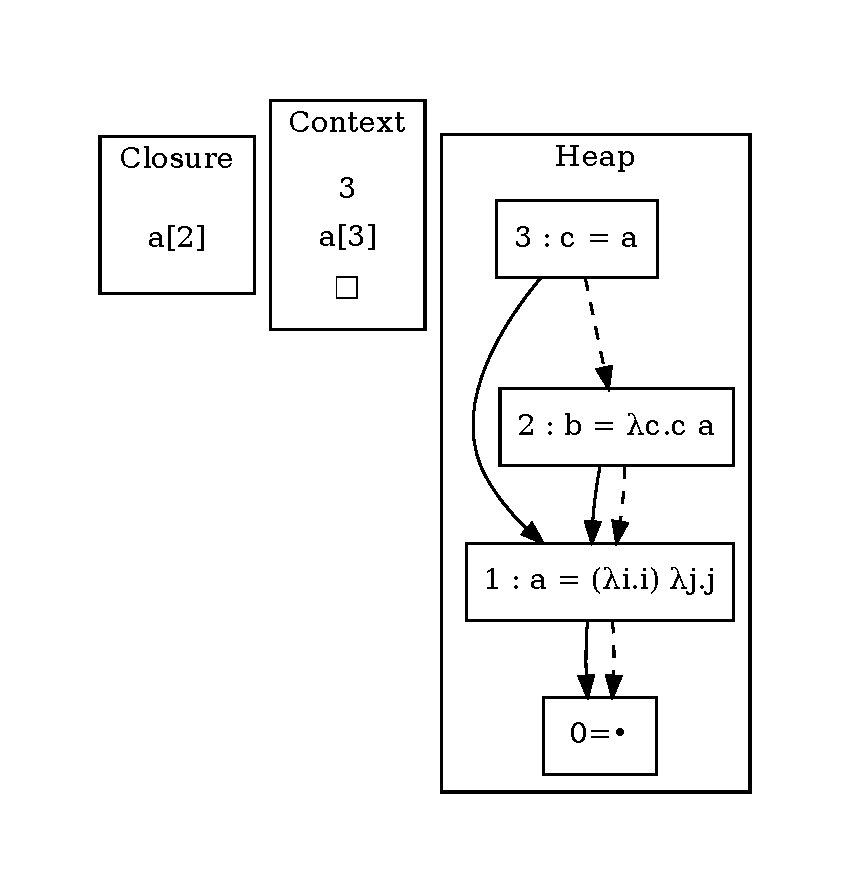
\includegraphics[width=\linewidth/2]{figures/11.pdf}
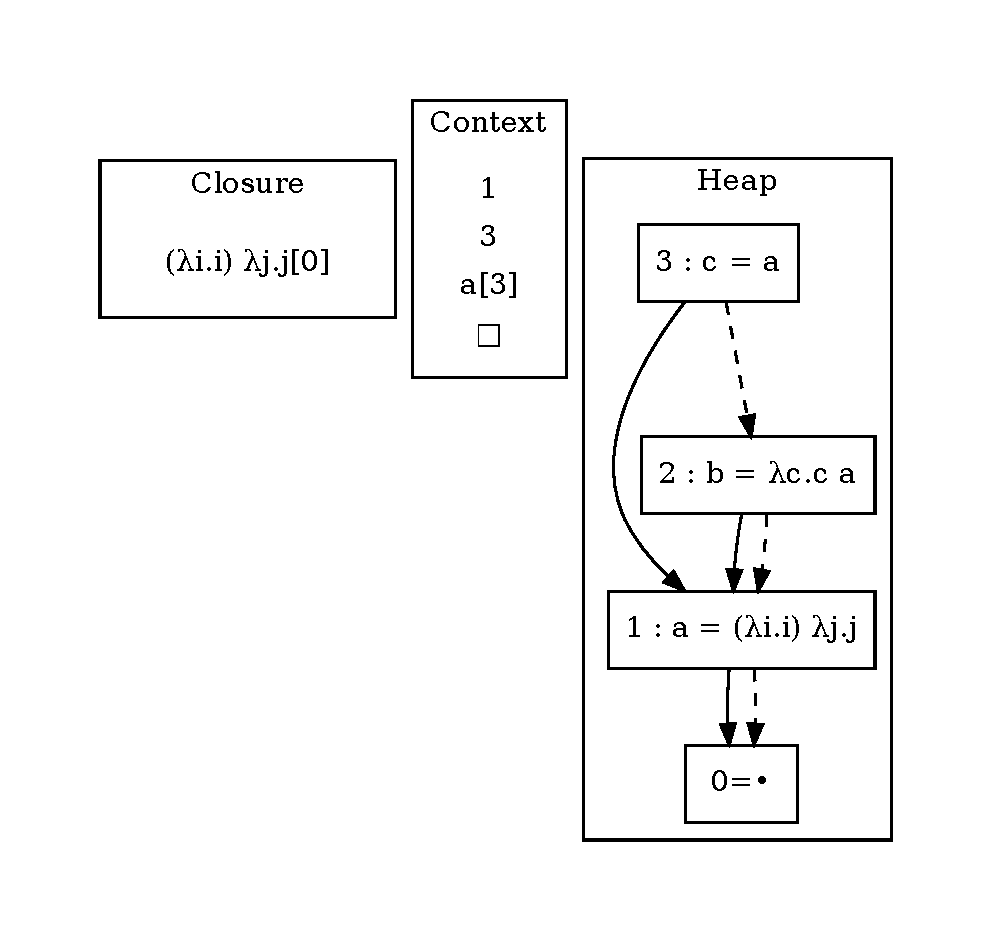
\includegraphics[width=\linewidth/2]{figures/12.pdf}
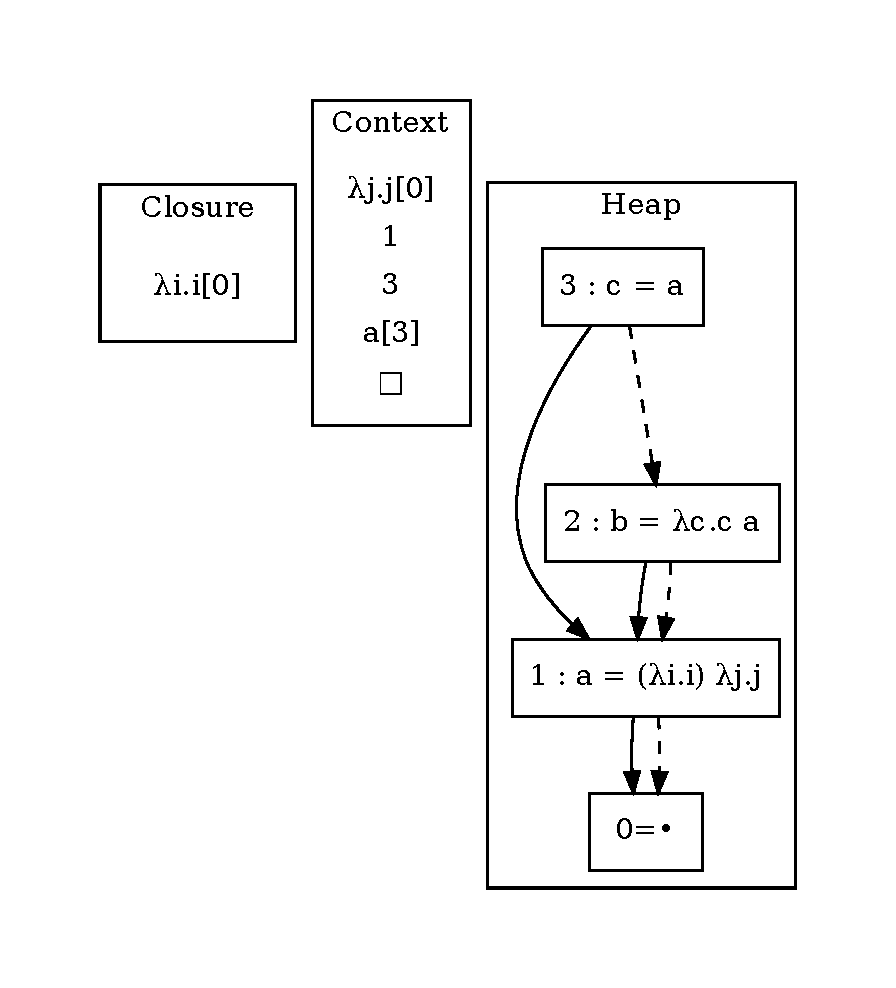
\includegraphics[width=\linewidth/2]{figures/13.pdf}
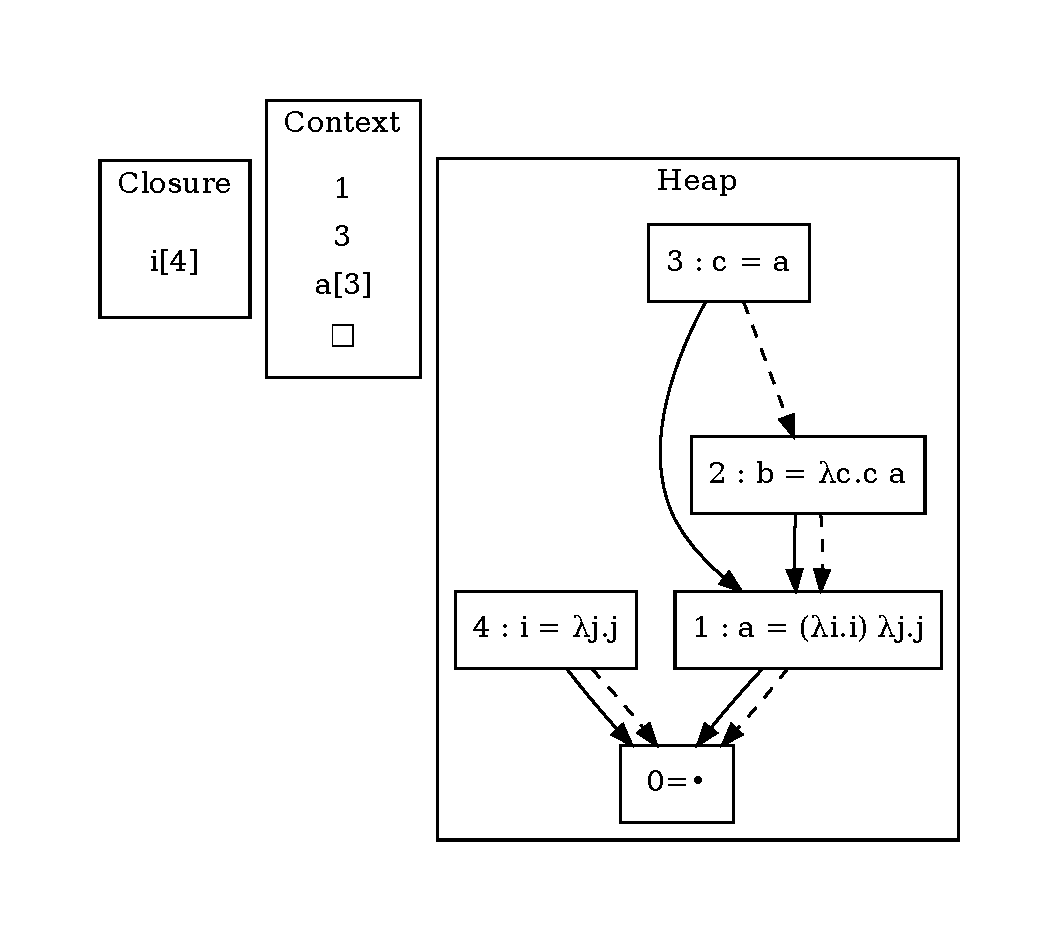
\includegraphics[width=\linewidth/2]{figures/14.pdf}
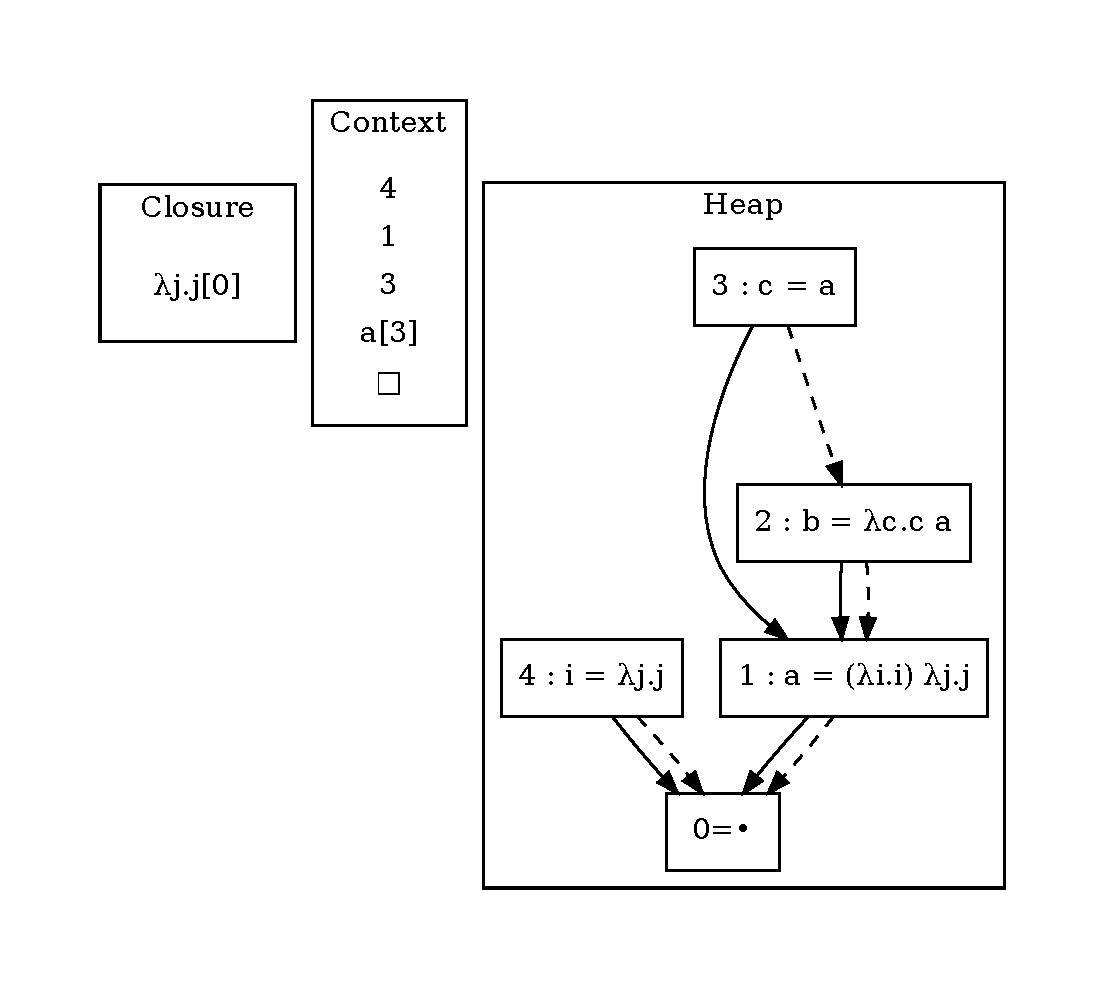
\includegraphics[width=\linewidth/2]{figures/15.pdf}
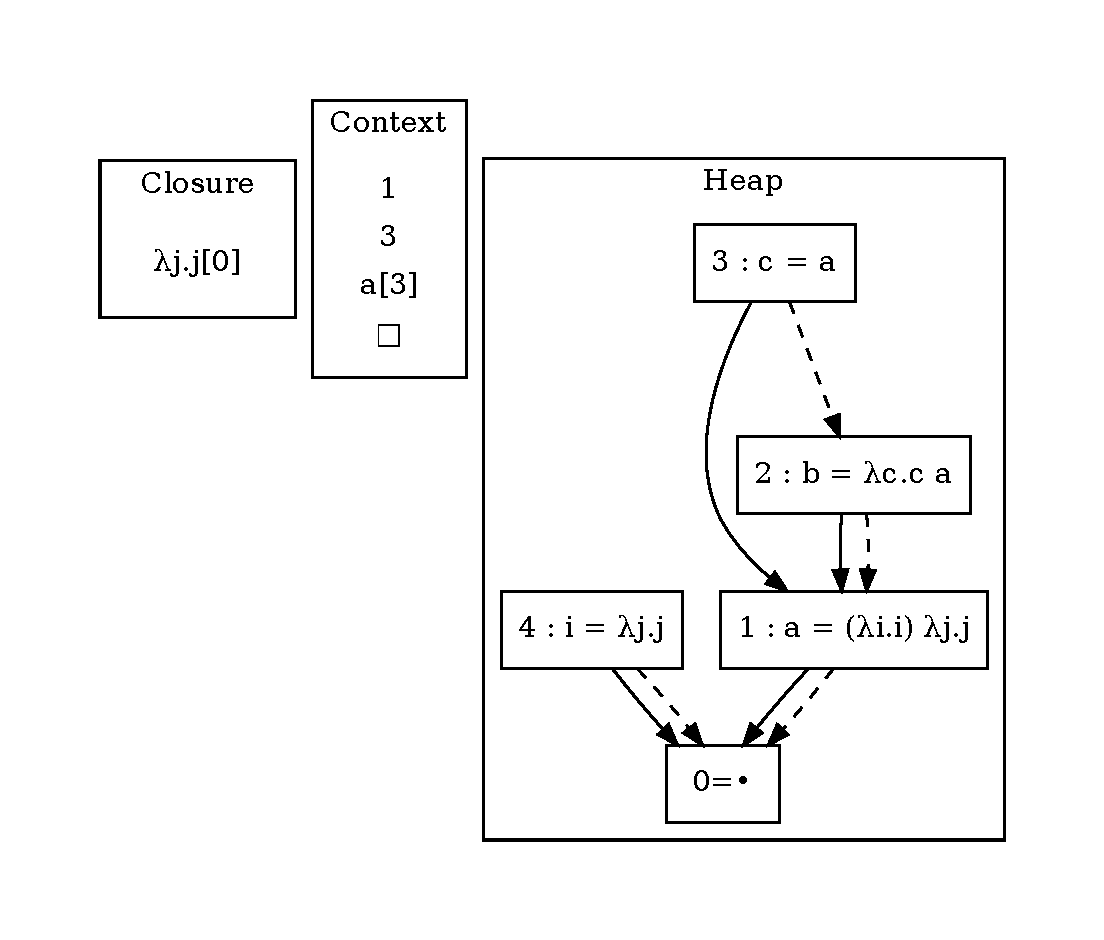
\includegraphics[width=\linewidth/2]{figures/16.pdf}
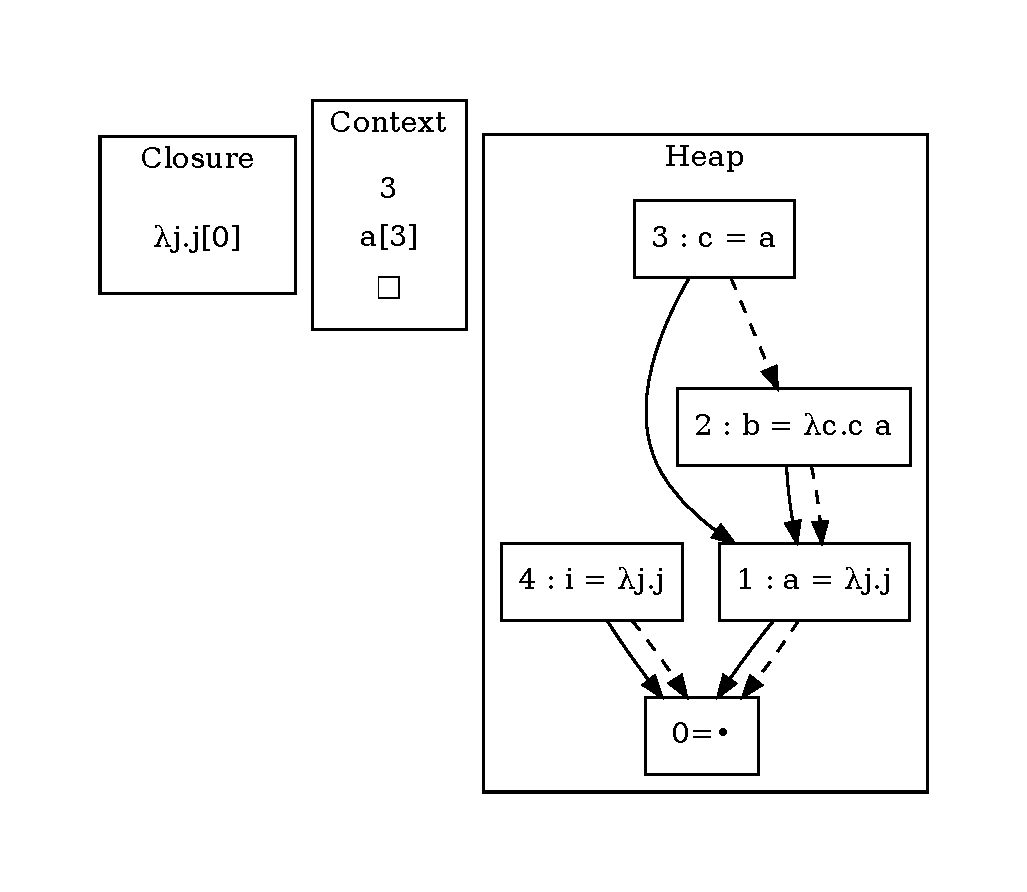
\includegraphics[width=\linewidth/2]{figures/17.pdf}
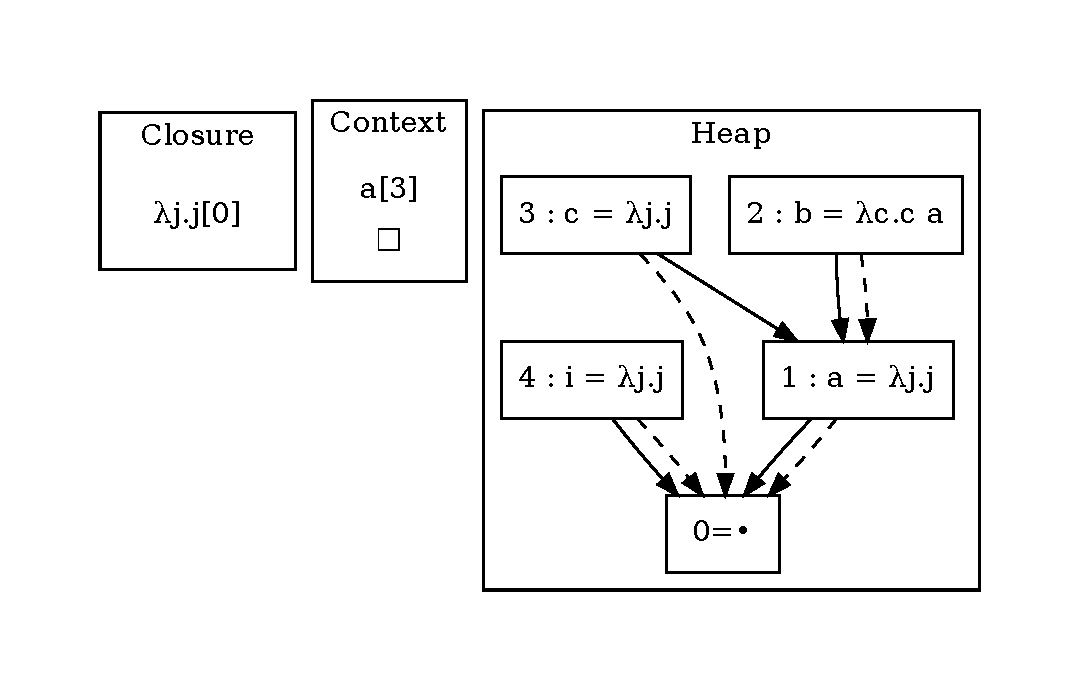
\includegraphics[width=\linewidth/2]{figures/18.pdf}
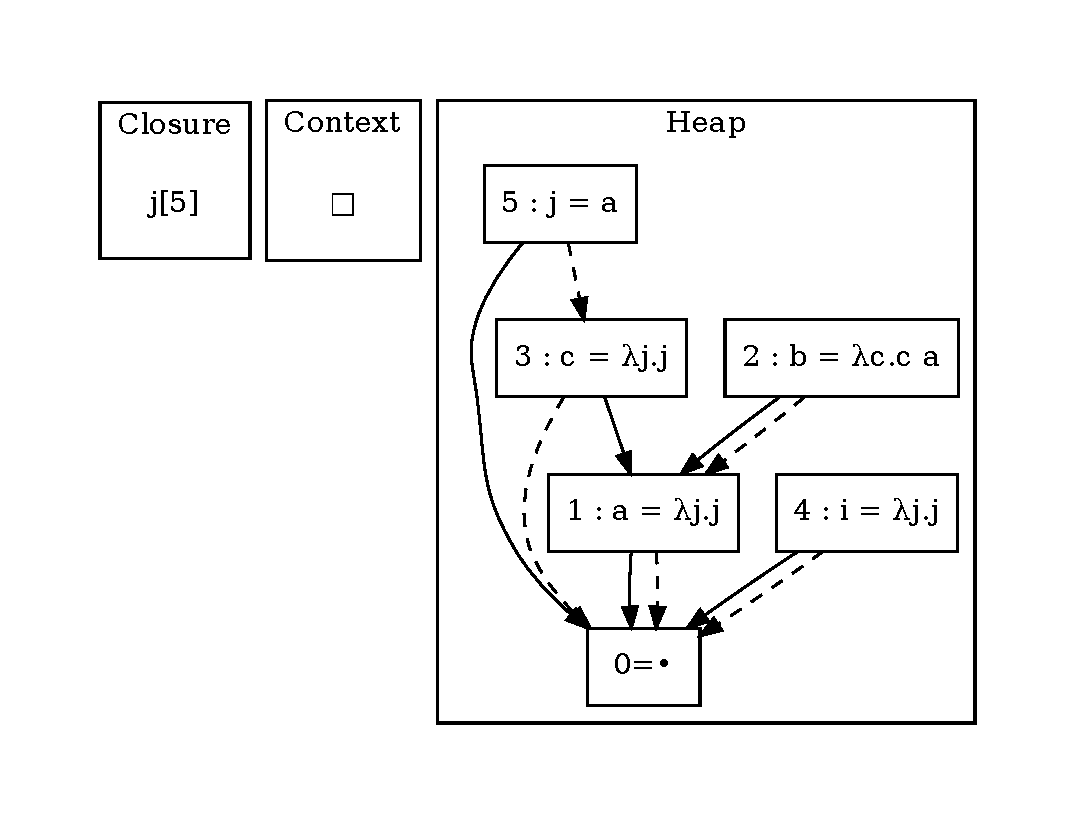
\includegraphics[width=\linewidth/2]{figures/19.pdf}
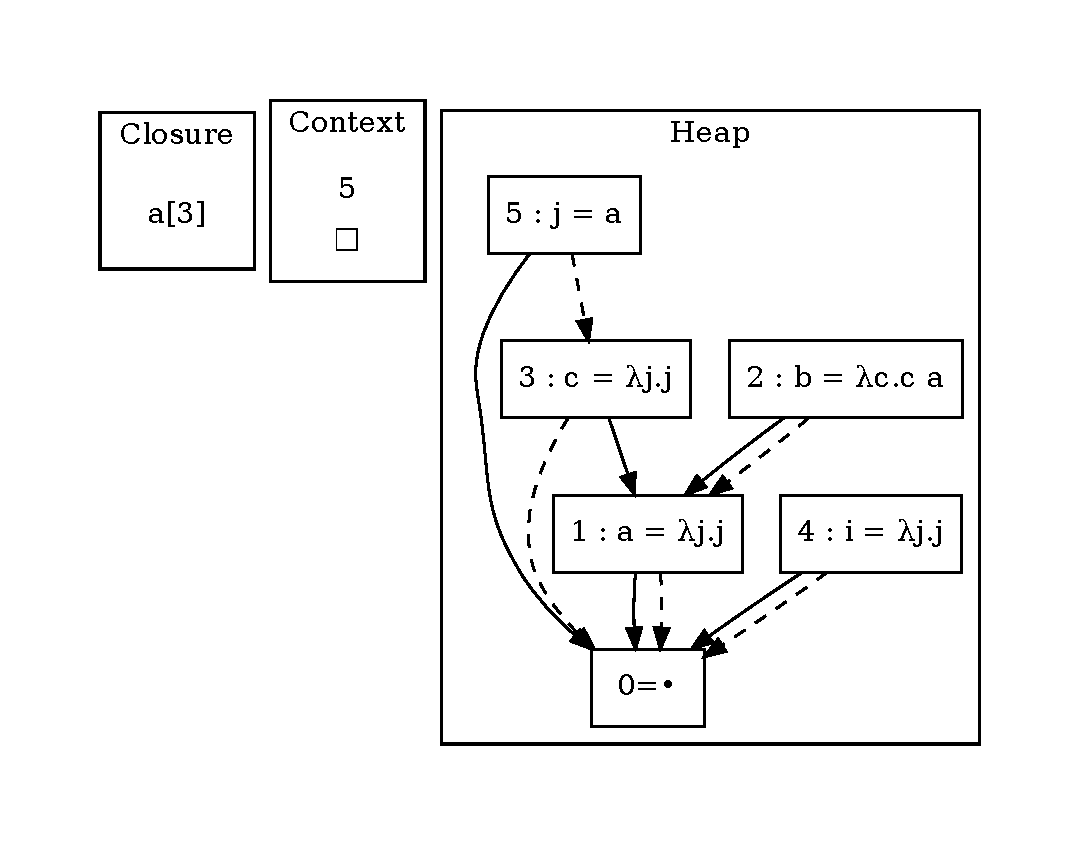
\includegraphics[width=\linewidth/2]{figures/20.pdf}
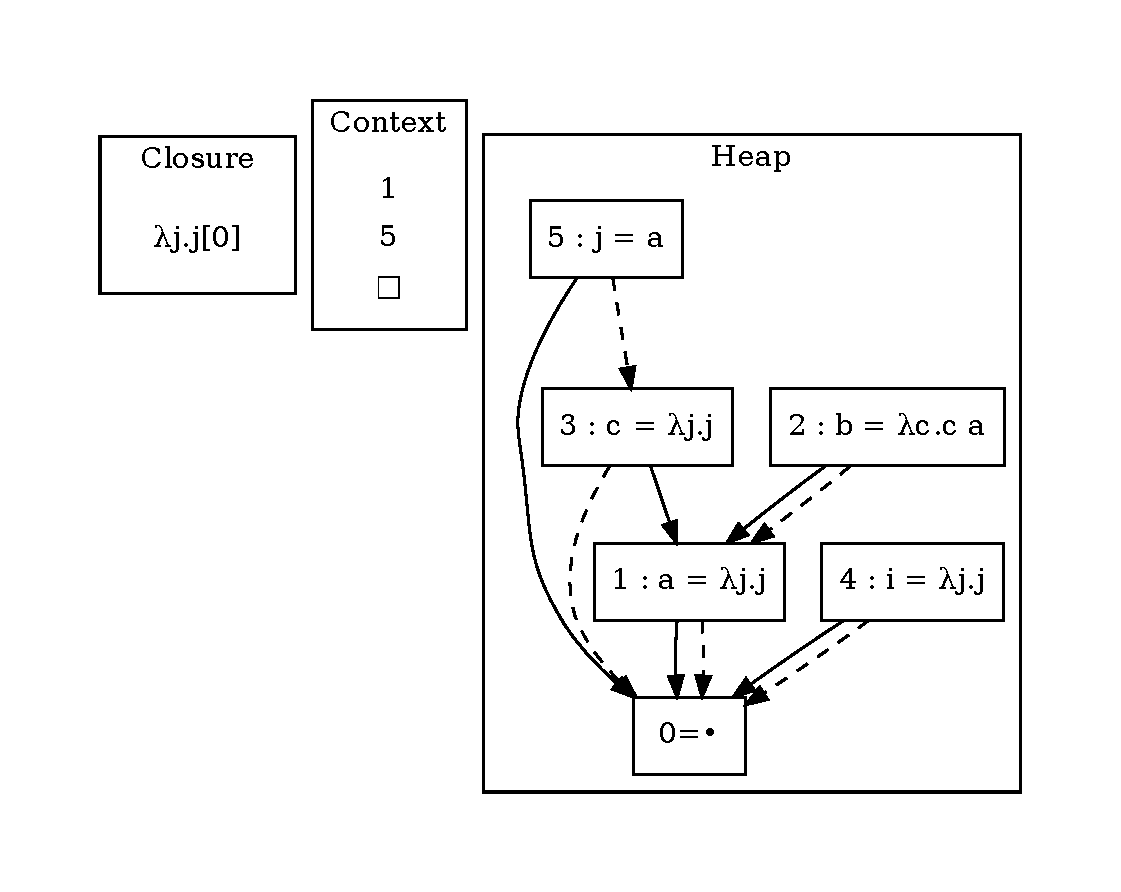
\includegraphics[width=\linewidth/2]{figures/21.pdf}
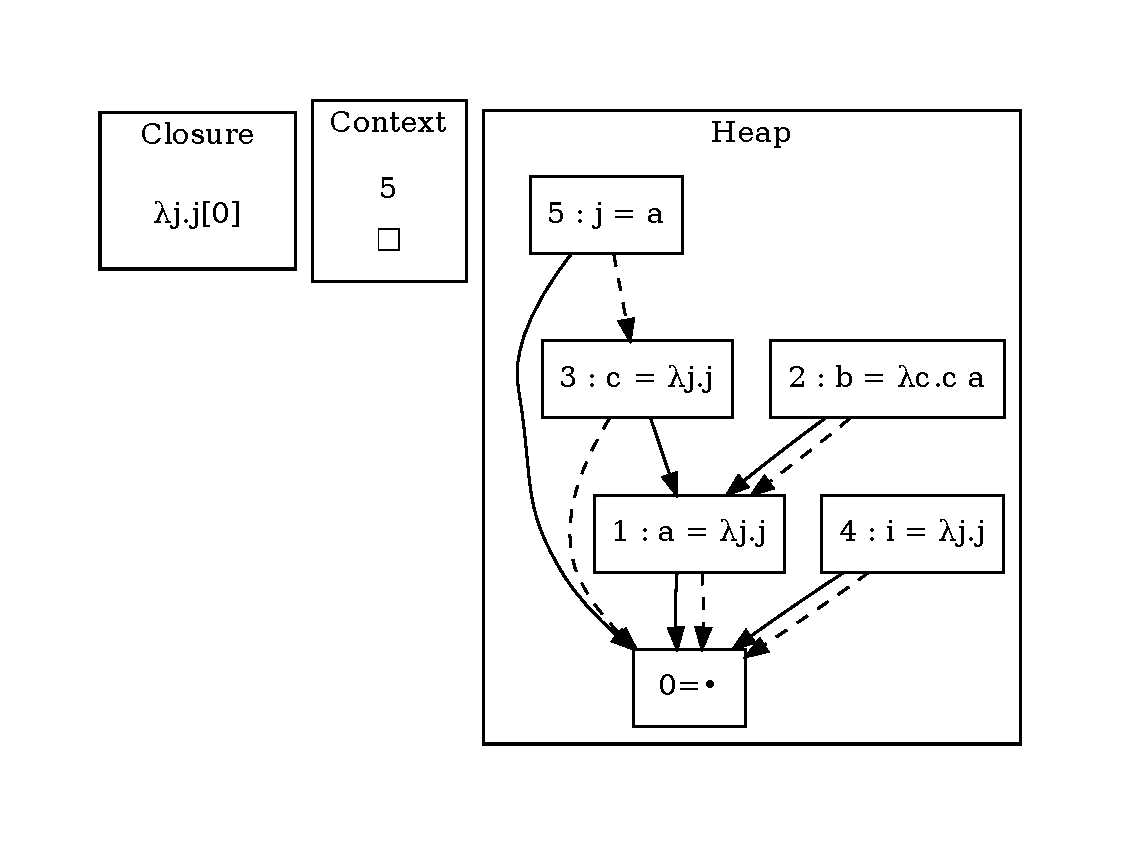
\includegraphics[width=\linewidth/2]{figures/22.pdf}
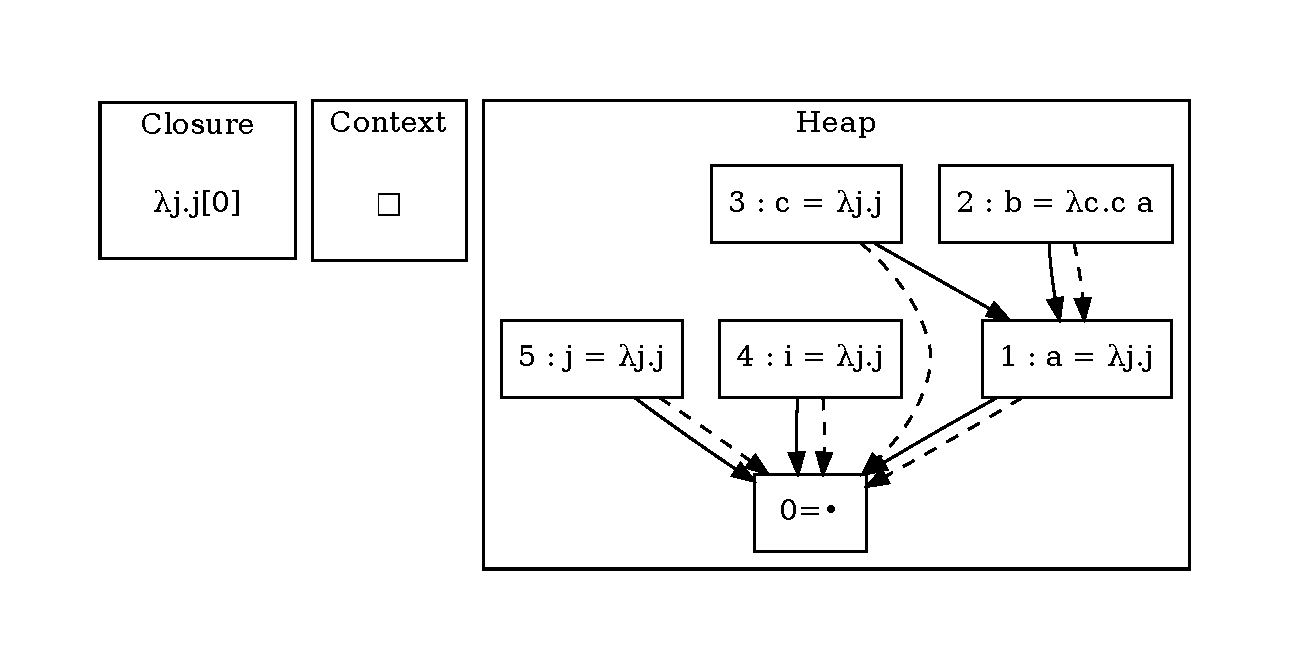
\includegraphics[width=\linewidth/2]{figures/23.pdf}

We can see that through the evaluation, the variable \texttt{a} is dereferenced
twice, in two different scopes. The cactus structure ensures that the value is
correctly shared between the two instances, with the second dereference
correctly dereferencing the evaluated identity function. 

